\chapter{Performance analysis}

The following chapter presents the results of performance analysis of Translation and Interpretation CPU simulators,
and compares the performance of different solutions. The first section of this chapter focuses
on the description of the test environment in terms of hardware, software, and simulated guest parameters and
characteristics. The second section describes the benchmarks and binaries and motivates their importance in the field
of automatics and robotics, especially in the context of Industry 4.0. The last section presents and interprets
the results.

\section{Test enviroment}
In order to achieve representative and reproducible results, the test environment must be carefully controlled, as not
to introduce any inaccurate and misleading conclusions. All of the tests were performed on the following testbench:

\begin{table}[h!]
    \centering
    \begin{tabular}{l|l}
    CPU              & Intel(R) Core(TM) i7-8700             \\
    \hline
    Memory           & 32GB DDR4 @ 2133 Mhz                  \\
    \hline
    Operating System & Linux Fedora 36 (6.0.9-200)           \\
    \hline
    C stdlib         & GNU libc 2.35                         \\
    \hline
    .NET Runtime     & Mono JIT compiler version 6.12.0.122
    \end{tabular}
\end{table}

\noindent
In terms of software, both Renode Translation Libraries and Dromajo are compiled using the \texttt{-O3} optimization
level. In addition to that, the libraries are \textbf{not using} any architecture specific optimizations:
they were compiled \textbf{without} \texttt{-march=native} and \texttt{-mtune=native} flags. This is an important
to note, as using these flags might significantly improve the overall performance of simulators, but since
this work only focuses on performance deltas, these flags do not provide any additional value, and in the worst
case might introduce unwanted behavior.

The simulated guest platform is \textbf{BeagleV Starlight JH7100}, with the only difference between the benchmark test
cases being the used CPU emulator.

In order to provide deterministic results, every test case is performed with the \textbf{SetGlobalSerialExecution}
flag set to true. This Renode setting forces emulated processors to perform sequentially, removing the variability
introduced by the host operating system scheduler, thus maintaining full determinism.

\pagebreak

\section{Benchmark payloads and tested parameters}

\begin{itemize}
    \item{\textbf{Zephyr RTOS boot-up routine} this test runs a Zephyr RTOS payload boot-up sequence and waits for
    a 'hello-world' messeage on a UART device \cite{ZephyrHello}.\\
    \textbf{Motivation:} This test will determine whether the performance benefits/detriments are noticeable when
    running a very simple payload. This is important as the current trend in the industry heads in the
    direction of implementing decentralized IoT and edge computing solutions, often using cheaper and
    smaller devices running leaner payloads.}
    %
    \item{\textbf{Zephyr RTOS $\pi$ calculating sample} This sample application calculates the value of $\pi$ independently in many
    threads, and demonstrates the benefit of multiple execution units (CPU cores) when compute-intensive tasks can be
    run in parallel, with no cross-dependencies or shared resources \cite{ZephyrPi}.\\
    \textbf{Motivation:} In the context of Industry 4.0, this payload might represent the arithmetic operations
    performed while calculating an advanced automatic control system, or other algorithmically and/or numerically
    advanced tasks.}
    %
    \item{\textbf{Zephyr RTOS TensorFlow Lite Micro Module} this test runs the TensorFlow Lite Micro Zephyr module,
    runs the ML model, and waits for it to finish. The model included with the sample is trained to replicate a sine
    function and generates x values to print alongside the y values predicted by the model. X values iterate from 0
    to an approximation of 2$\pi$ \cite{ZephyrTF}.\\
    % DNN? Isn't it safer to write ML?
    \textbf{Motivation:} A lot of the Industry 4.0 endpoints, such as sensors and actuators, use simple AI/DNN
    deployments, either to prematurely filter collected data or to assist in decision-making. The proposed sample
    is a good match, as the neural network is not overly complicated, and runs on a real-time operating system.}
    %
    \item{\textbf{Linux kernel boot-up} this test loads all necessary payloads to boot the Linux kernel.\\
    As the Linux kernel is a relatively complicated payload, this test checks a wide range of the CPU simulation use
    cases\\
    % Unreapeatable?
    \textbf{Motivation:} In Industry 4.0 times, the Linux kernel had become an unrepeatable part of almost every
    automatic control, internet of things, robotics, etc. infrastructure stack. Because of that it is important to
    provide a qualitative and performance evaluation of the simulation.}
\end{itemize}

\noindent
Each test was repeated three times, and evaluated under the following criteria:
\begin{itemize}
    \item{\textbf{Qualitative evaluation}, has the test finished successfully and returned correct data?\\
    Verified on a case-by-case basis.}
    %
    \item{\textbf{Performance evaluation}, how long did the test take?\\To guarantee accuracy and validity, this metric is
     provided by Renode Virtual Time framework.}
\end{itemize}

\pagebreak

\section{Benchmark results}

Plots below are created by performing each benchmark three times, the bar value represents the mean, with the error bars
representing standard deviation. These characteristics have also been provided in text form below the plot. The
\texttt{1c} and \texttt{2c} in the chart title represent number of virtual cores used when performing the test.

\subsection{Zephyr RTOS boot-up routine}

\begin{figure}[h]
	\centering
	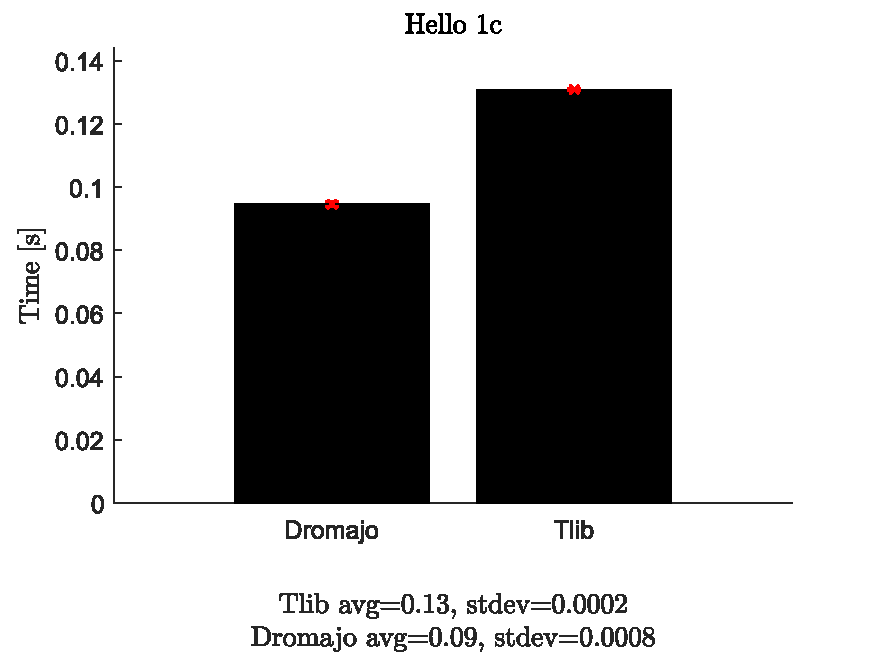
\includegraphics[width=0.6\textwidth]{figures/benchmarks/Hello1c.pdf}
	\caption{Zephyr RTOS boot times}
\end{figure}
\noindent
\textbf{Qualitative evaluation}: Both simulators were able to correctly boot up Zephyr RTOS.
\vspace*{15px}

\subsection{Zephyr RTOS $\pi$ calculating sample}

\begin{figure}[h]
    \centering
    \begin{subfigure}{0.5\textwidth}
      \centering
      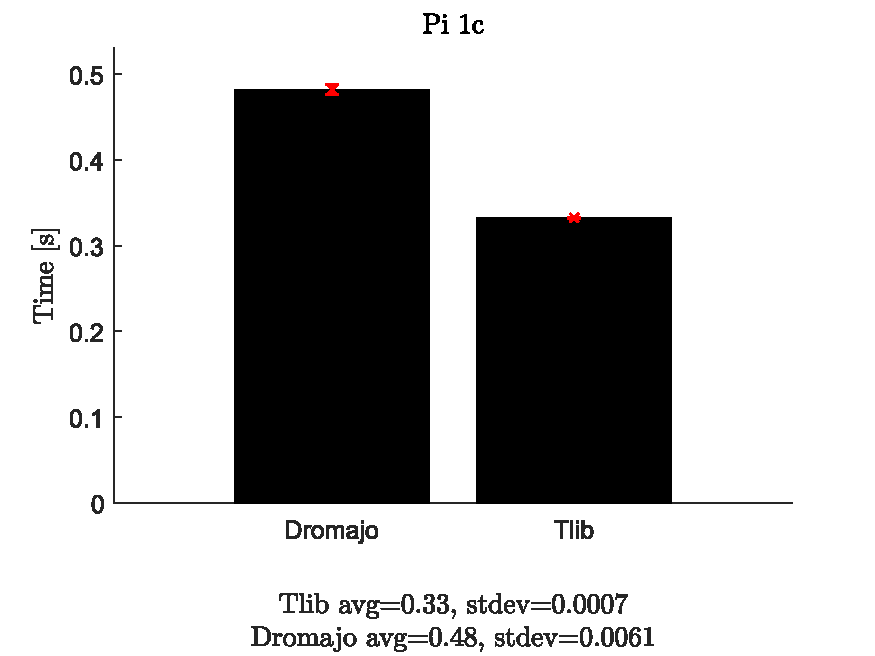
\includegraphics[width=1.2\linewidth]{figures/benchmarks/Pi1c.pdf}
    \end{subfigure}%
    \begin{subfigure}{0.5\textwidth}
      \centering
      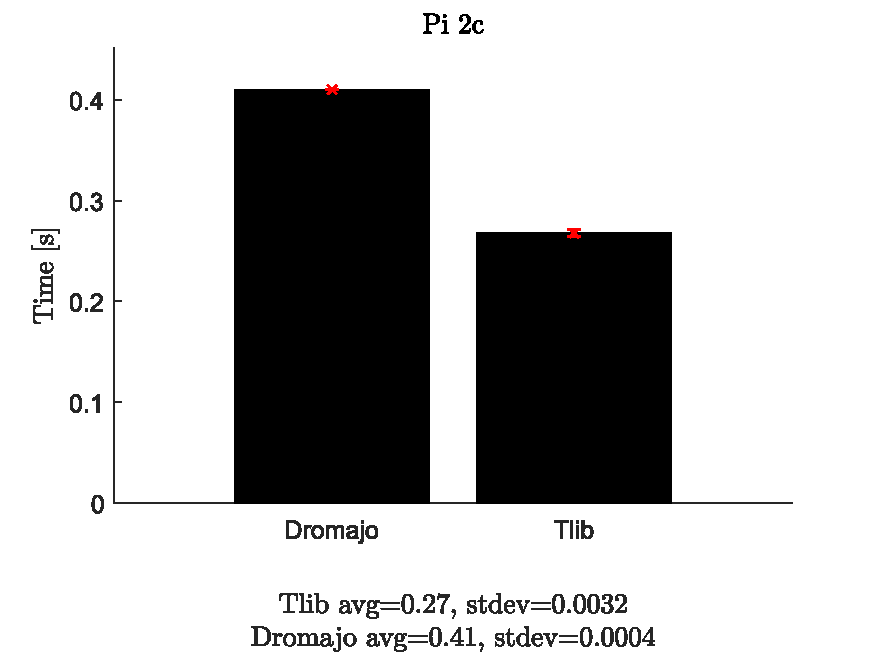
\includegraphics[width=1.2\linewidth]{figures/benchmarks/Pi2c.pdf}
    \end{subfigure}
    \caption{Zephyr RTOS $\pi$ calculating times}
\end{figure}
\textbf{Qualitative evaluation}: Both simulators have correctly executed the algorithm.
%Frankly speaking, I feel these will be much better if they had the samy Y scale... That applies to all 1c/2c graphs

\pagebreak

\subsection{Zephyr RTOS TensorFlow Lite Micro Module}

\begin{figure}[h]
    \centering
    \begin{subfigure}{0.5\textwidth}
      \centering
      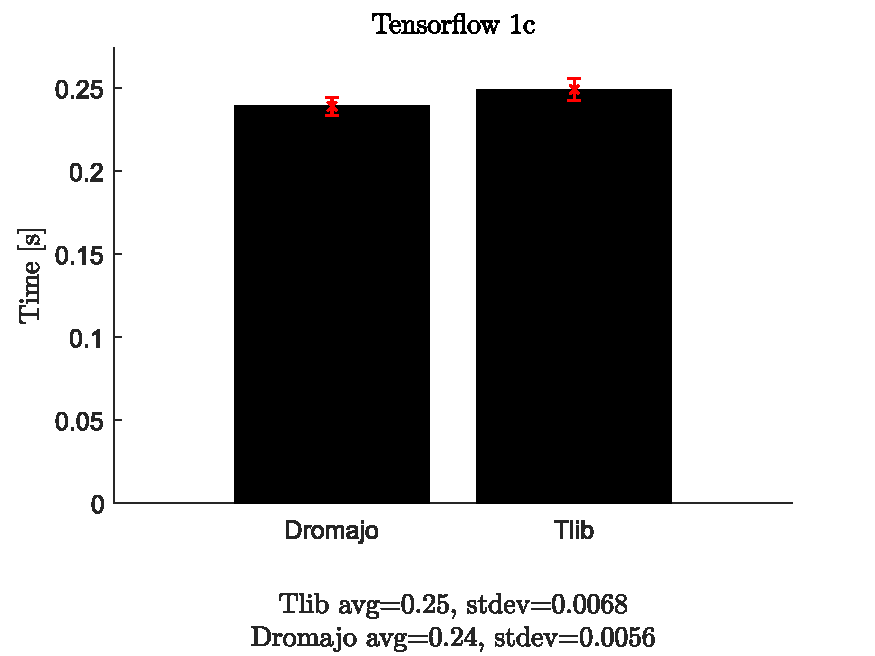
\includegraphics[width=1.2\linewidth]{figures/benchmarks/Tensorflow1c.pdf}
    \end{subfigure}%
    \begin{subfigure}{0.5\textwidth}
      \centering
      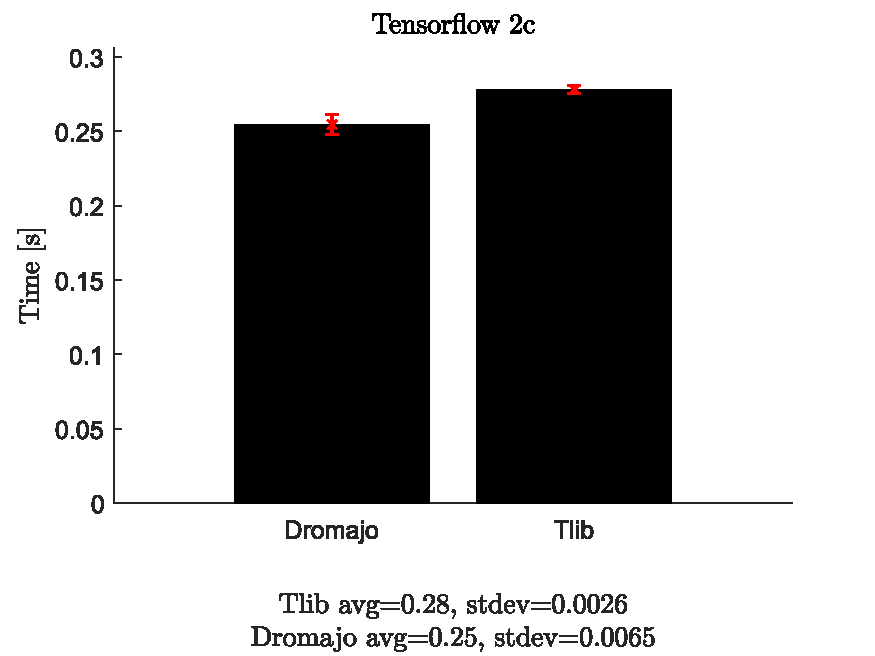
\includegraphics[width=1.2\linewidth]{figures/benchmarks/Tensorflow2c.pdf}
    \end{subfigure}
    \caption{Zephyr RTOS Tensorflow execution time}
\end{figure}
\textbf{Qualitative evaluation}: Both simulators have correctly executed the algorithm.
\vspace*{15px}

\subsection{Linux kernel boot-up}

\begin{figure}[h]
    \centering
    \begin{subfigure}{0.5\textwidth}
      \centering
      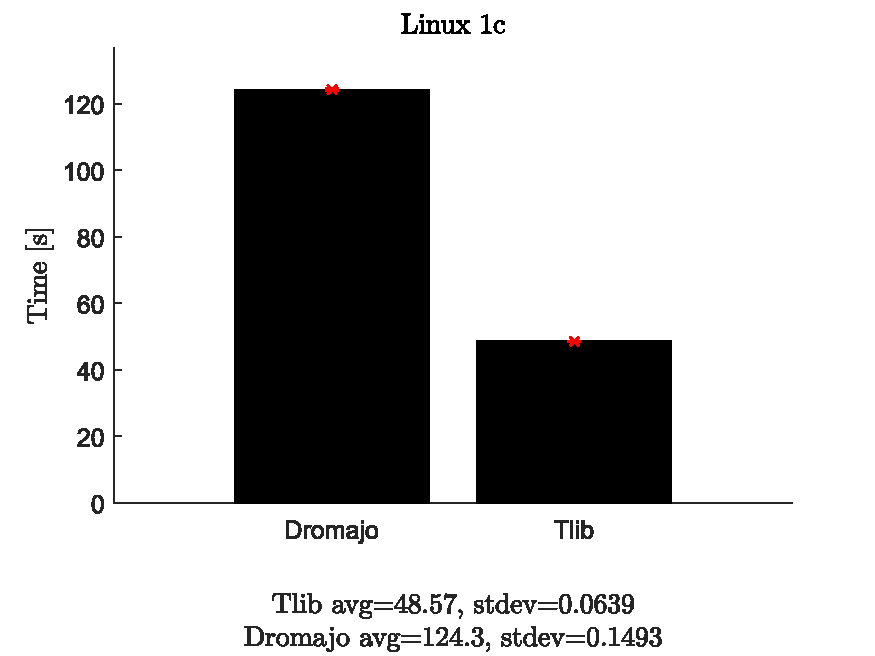
\includegraphics[width=1.2\linewidth]{figures/benchmarks/Linux1c.pdf}
    \end{subfigure}%
    \begin{subfigure}{0.5\textwidth}
      \centering
      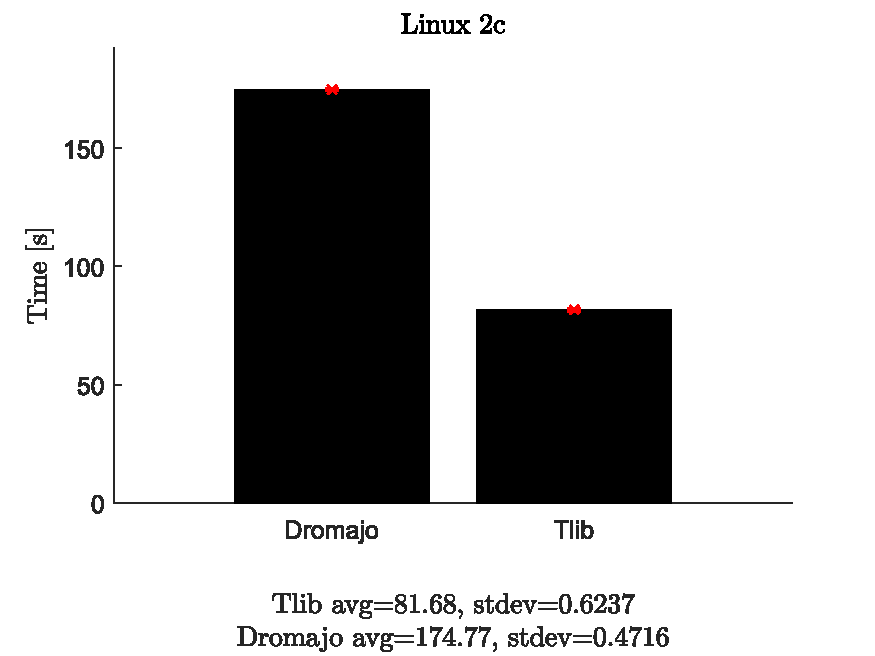
\includegraphics[width=1.2\linewidth]{figures/benchmarks/Linux2c.pdf}
    \end{subfigure}
    \caption{Zephyr RTOS Tensorflow execution time}
\end{figure}
\textbf{Qualitative evaluation}: Both simulators have correctly brought up the Linux kernel.
\vspace*{15px}

\noindent
The Linux kernel, being the biggest benchmark performed, generates a lot of logs on the UART console. This opened up a
possiblity to use Renode Log Tester to trace the time between each new message. This approach is called
\textit{Profiling} and is most typically used to perform a performance analysis for code execution. While some events
might be ommited (non-log emitting events), it is still an interesting data source that is worth investigating.

\pagebreak

\subsection{Linux boot profiling}
This section will provide two types of charts:
\begin{itemize}
    \item{\textbf{Boot profile chart}, a graph on a plane of virtual time versus host time. Each point represents a
    UART console message at a given point in time. This plot represents two pieces of information, the cumulative
    speedup or slowdown and the rate of change of the beforementioned characteristic. The increasing slope means that
    simulating the virtual processor, at this point, takes more time than is passing in real time. The decreasing slope
    represents the case when the simulated CPU is executing instructions faster than real time. If the chart slope
    matches the gray line slope, the simulated processor is executing instructions at exactly realtime speed.
    The gray line represents the "one-to-one" time mapping. If the execution chart is above this line, this means
    that the virtual CPU is lagging behind the real time and vice versa.}
    %
    \item{\textbf{Cumulative speedup chart}, provides a normalised version of the boot profile chart.
    The gray y-axis line represents "one-to-one" time mapping, with the same interpretation as in the boot profile
    chart.}
\end{itemize}

\pagebreak

%This graph is not readable! Really, even on serious zoom. I suggest rotating it clockwise 90 deg and increasing fonts
% also what is ioaccesses? I would also add the "prompt" event
\subsection*{Linux boot profiling - Tlib}
\begin{figure}[h]
	\centering
    \hspace*{-2cm}
	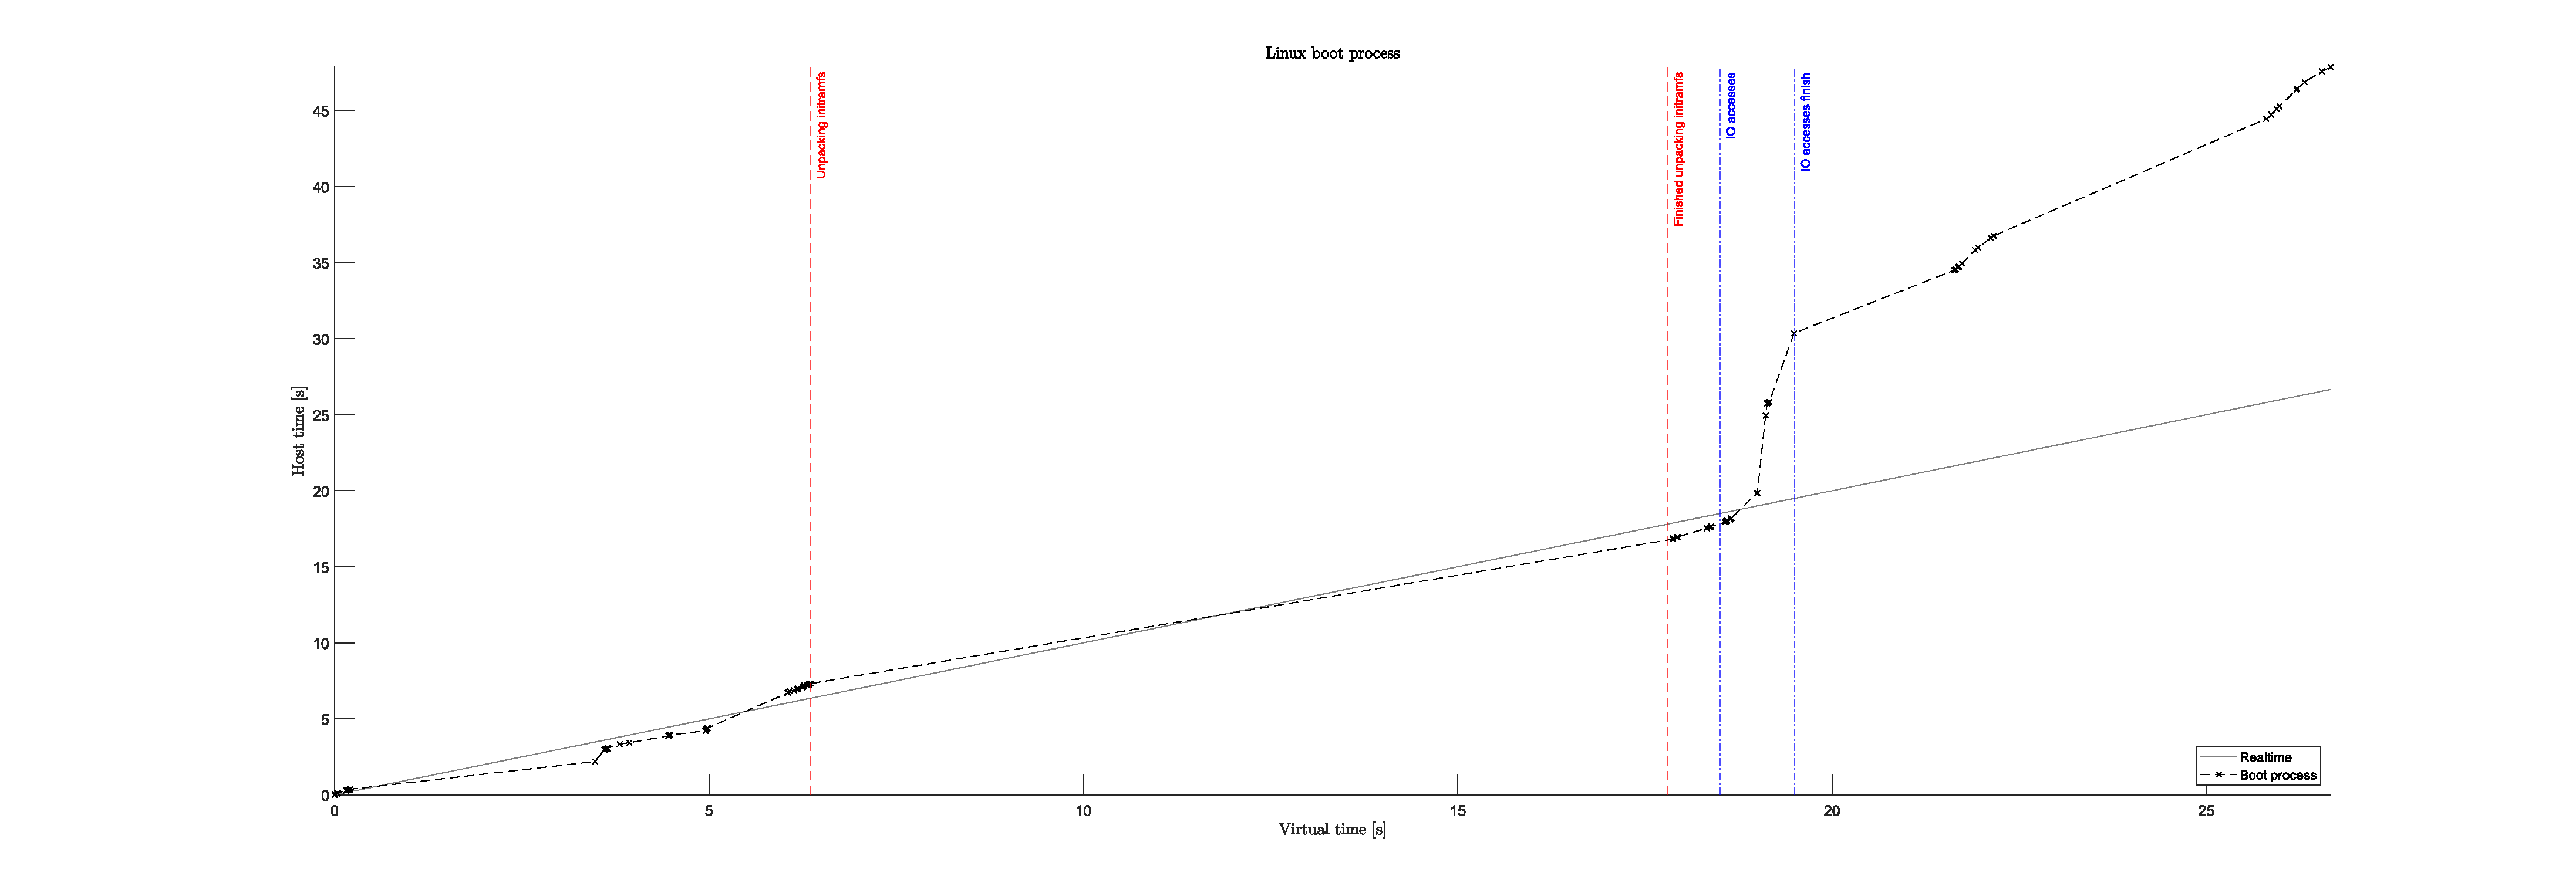
\includegraphics[width=1.2\textwidth]{figures/benchmarks/linux_boot/adnotated/TlibBoot.pdf}
	\caption{Linux boot profile chart - Translation Libraries}
\end{figure}

\noindent
The translation-based CPU was able to maintain a one-to-one virtual host time relation for most of
its execution, only falling behind when the I/O devices were heavily accessed. This is expected, as this mode of memory
access is not a subject to optimization methods described in the Chapter 3. Additionally, these accesses require a C
$\rightarrow$ C\# callback, which is also noticeably slow. After these accesses have been completed, the slope of the
chart returns to almost realtime, but not quite reaching it.

The area bounded by the red markers represents the time when the Linux kernel payload was unpacking initramfs. In terms
of the Linux kernel, this means extracting the initialization utilities from the \textit{gzip} archive into the
device random access memory, allowing the kernel to use RAM as a temporary rootfs. Since the boot process is not
progressing any further, it is not sending any messages to the UART device, thus expalining the lack of the data
points.

% same as above
\begin{figure}[h]
	\centering
    \hspace*{-2cm}
	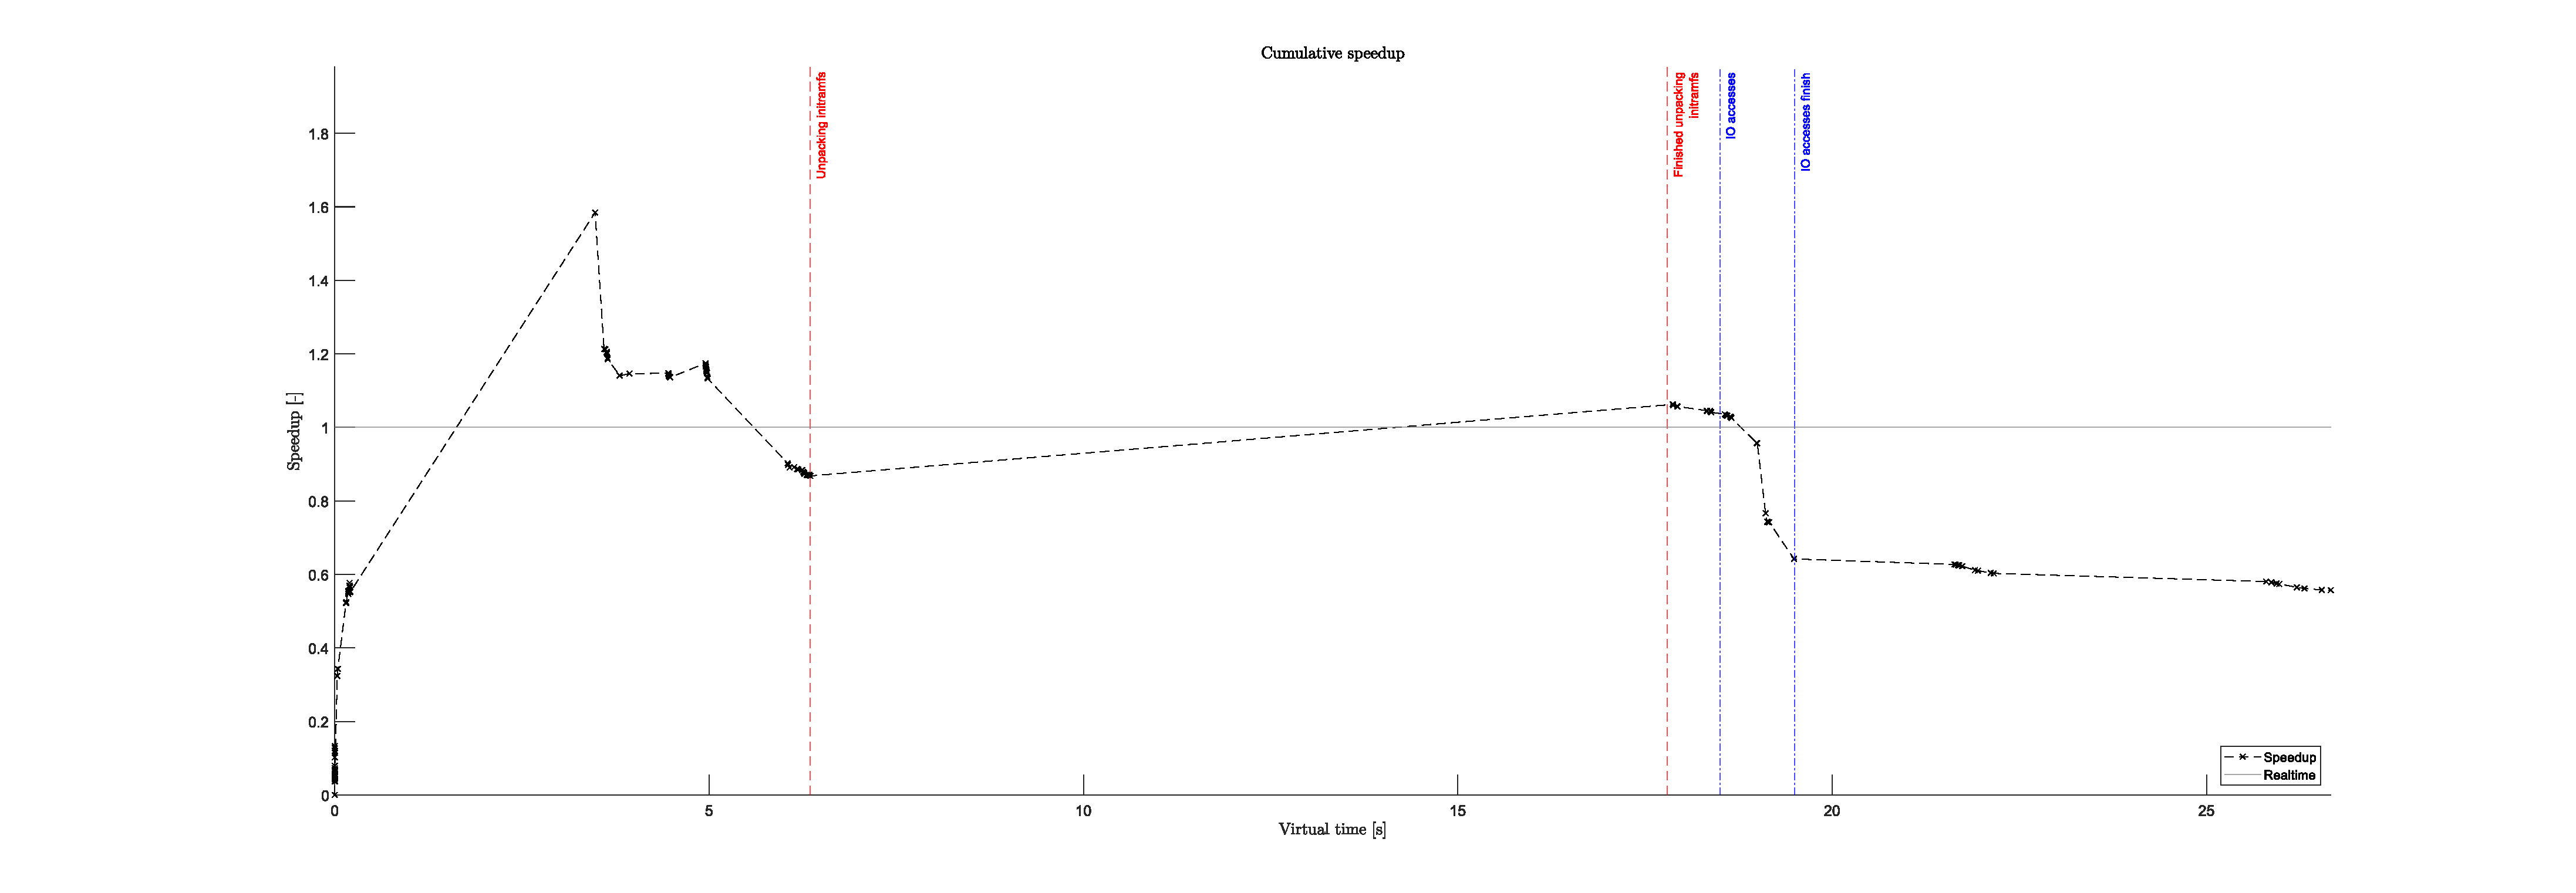
\includegraphics[width=1.2\textwidth]{figures/benchmarks/linux_boot/adnotated/TlibSpeedup.pdf}
	\caption{Linux speedup chart - Translation Library}
\end{figure}

\pagebreak

\subsection*{Linux boot profiling - Dromajo}

\begin{figure}[h]
	\centering
    \hspace*{-2cm}
	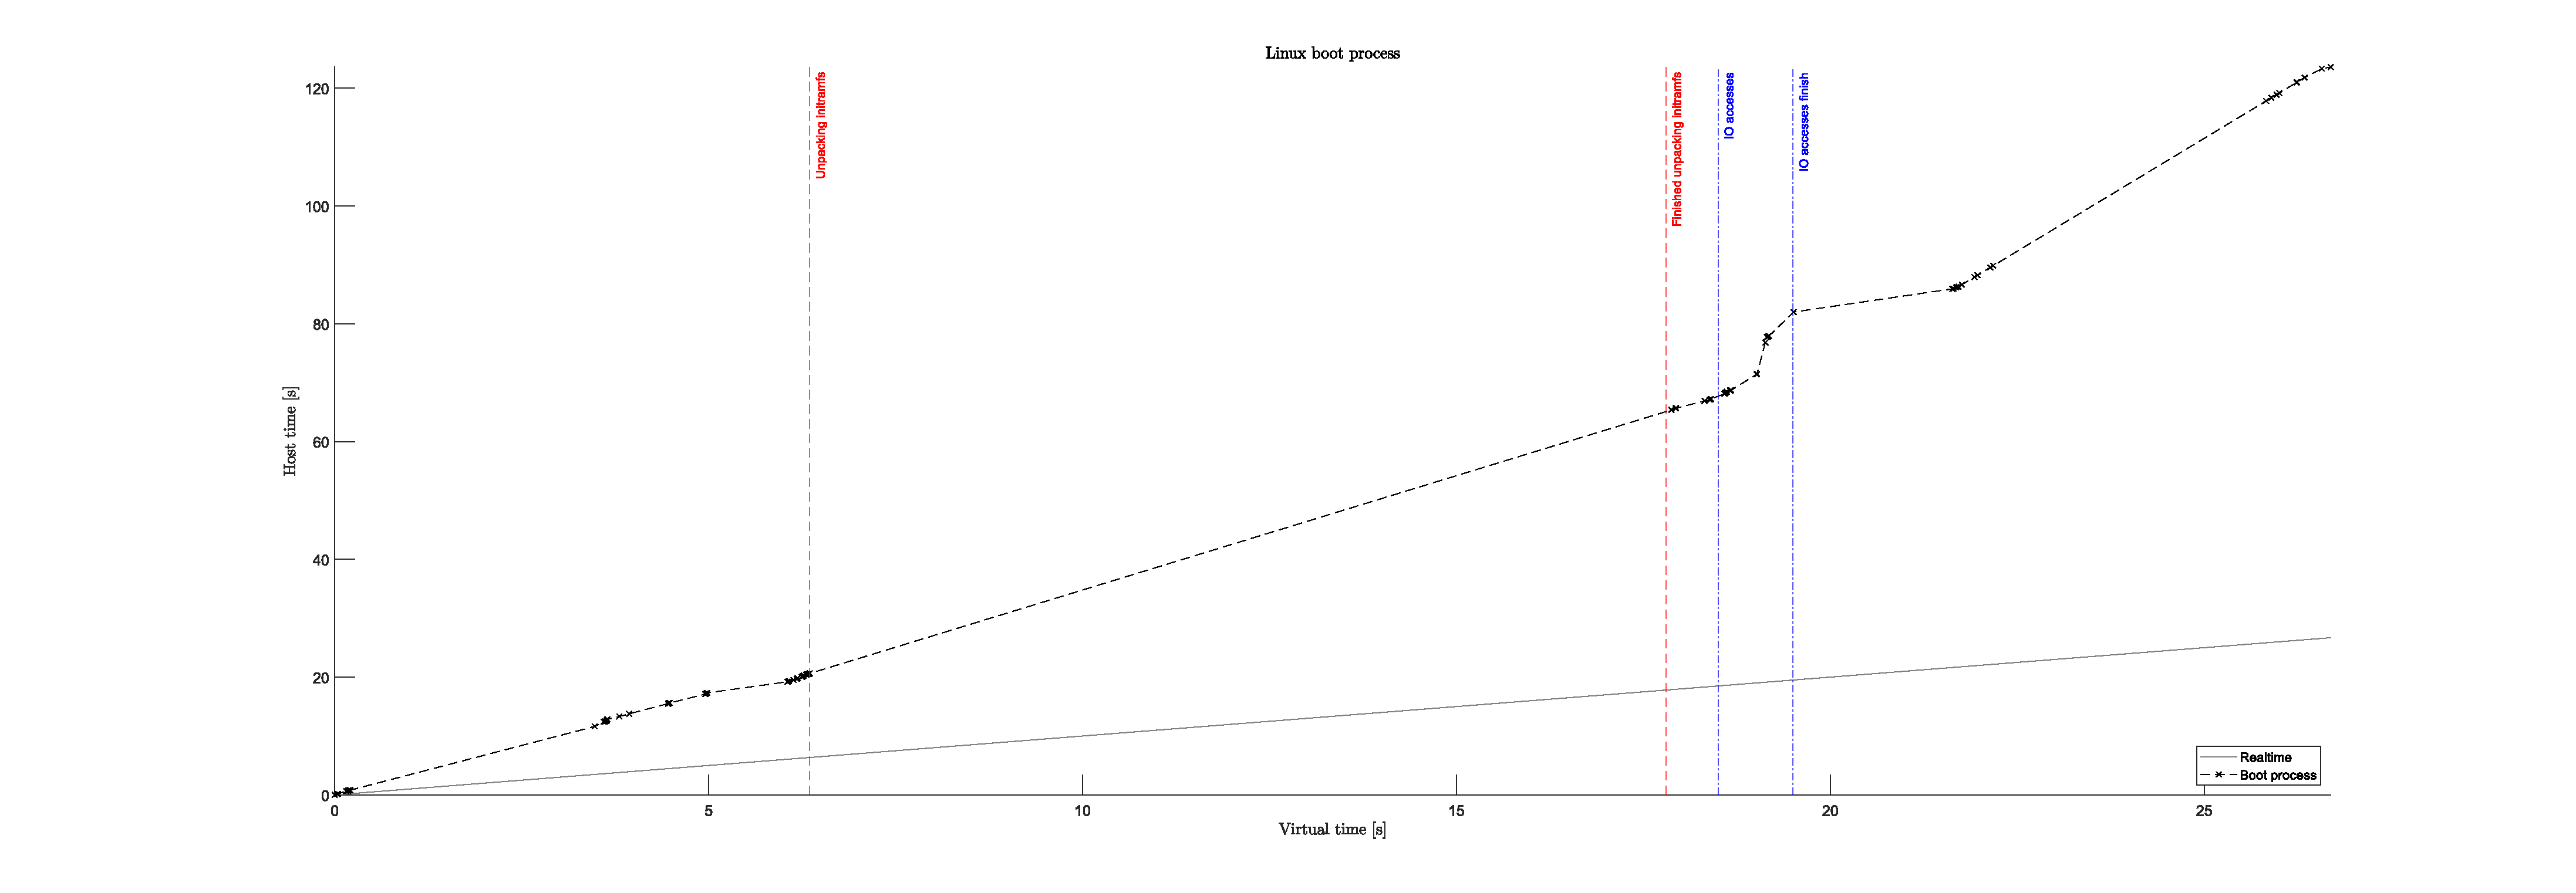
\includegraphics[width=1.2\textwidth]{figures/benchmarks/linux_boot/adnotated/DromajoBoot.pdf}
	\caption{Linux boot profile chart - Dromajo}
\end{figure}

\noindent
The Dromajo simulated CPU was not able to maintain a one-to-one virtual host time relation, it has immediately fallen
behind the real time execution. The characteristics of the chart are the same as in the Translation Libraries case, but the
%but the speedup graph is always much lower than one?
execution slope is always much bigger than one.

\begin{figure}[h]
	\centering
    \hspace*{-2cm}
	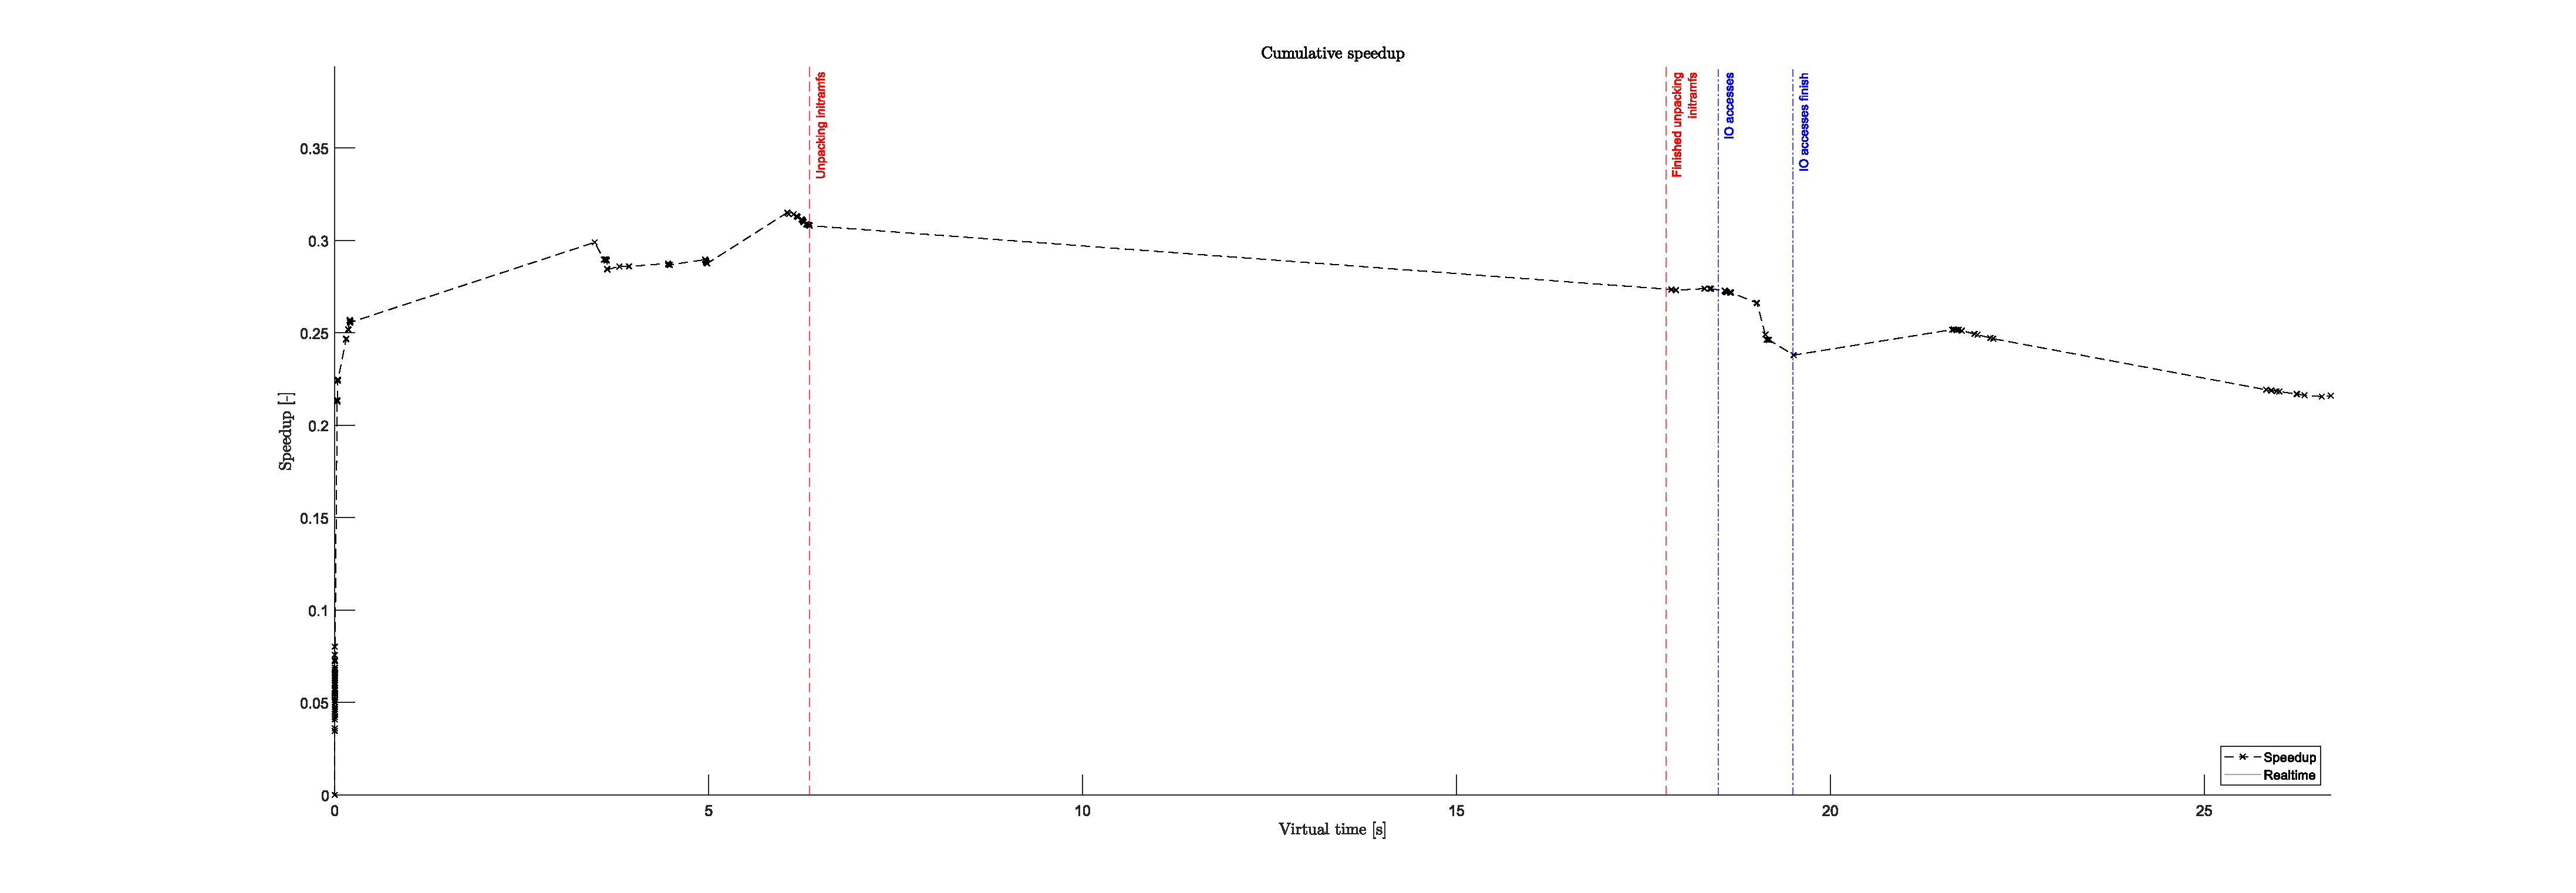
\includegraphics[width=1.2\textwidth]{figures/benchmarks/linux_boot/adnotated/DromajoSpeedup.pdf}
	\caption{Linux speedup chart - Dromajo}
\end{figure}

\pagebreak

\section{Performance conclusions}

\begin{table}[h]
    \centering
    \begin{tabular}{l|l|l}
    Benchmark             & Translation Libraries & Dromajo  \\ \hline
    Zephyr boot-up        & 0.13                  & 0.09     \\ \hline
    Zephyr $\pi$ calculation & 0.33               & 0.48     \\ \hline
    Zephyr Tensorflow     & 0.25                  & 0.24     \\ \hline
    Linux kernel boot-up  & 45.57                 & 124.3
    \end{tabular}
    \caption{Benchmark summary results for single core tests}
\end{table}

\begin{table}[h]
    \centering
    \begin{tabular}{l|l|l}
    Benchmark             & Translation Library & Dromajo  \\ \hline
    Zephyr boot-up        & -                   & -        \\ \hline
    Zephyr $\pi$ calculation & 0.27                & 0.41     \\ \hline
    Zephyr Tensorflow     & 0.28                & 0.25     \\ \hline
    Linux kernel boot-up  & 81.68               & 174.77
    \end{tabular}
    \caption{Benchmark summary results for dual core tests}
\end{table}

\noindent
Both of the simulation methods managed to pass the qualitative evaluation. The virtual CPUs behaved in a stable
and expected way. A low standard deviation in both cases also confirms the stability and repeatability of the test
results.
%Standard deviation for 3 runs is... questionable. If someone asks you about it, you might be in trouble. Just saying.

In terms of performance, the Translation Library simulated central processing unit performs better at every more
complex test, by as much as two times in the Linux test. This behavior is a merit of the block caching and chaining,
exceptionally speeding up the simulation process. The techniques applied in this method of simulation allow the virtual
processor to reach near real time execution performance.

The Dromajo simulated CPU performed better in the simpler payloads, such as booting the Zephyr RTOS, where the
optimization techniques used in the translation approach had become a noticeably big overhead - the process of
% This sentence is rewritable ;-)
block caching and chaining had significant cost and did not have any noticeable effect on the simulation, as it had
already ended. This suggests that for small payloads block caching and chaining is simply not a worthwile optimization
method.
